% Homecastr Investor Pitch Deck
% Compile with: pdflatex homecastr_pitch.tex

\documentclass[aspectratio=169,12pt]{beamer}

% ─── Theme & Colors ──────────────────────────────────────────
\usetheme{default}
\usecolortheme{default}
\setbeamertemplate{navigation symbols}{}
\setbeamertemplate{footline}{%
  \ifnum\thepage>1\relax%
    \hfill\usebeamercolor[fg]{page number in head/foot}%
    \usebeamerfont{page number in head/foot}%
    \insertframenumber\kern1em\vskip2pt%
  \fi%
}
\setbeamertemplate{frametitle}{
  \vspace{10pt}
  \begin{beamercolorbox}[wd=\paperwidth,center]{frametitle}
    \usebeamerfont{frametitle}\insertframetitle
    \par\vspace{4pt}
    {\color{hcGold}\hrule height 1.5pt width 4cm}
  \end{beamercolorbox}
}

% Homecastr brand palette — matches website beige theme
\definecolor{hcBg}{HTML}{F2EDE0}
\definecolor{hcText}{HTML}{3D3830}
\definecolor{hcGold}{HTML}{CA8A04}
\definecolor{hcGoldLight}{HTML}{E8D5A0}
\definecolor{hcMuted}{HTML}{7E7B74}
\definecolor{hcCard}{HTML}{EBE4D6}

\setbeamercolor{background canvas}{bg=hcBg}
\setbeamercolor{normal text}{fg=hcText}
\setbeamercolor{frametitle}{fg=hcText}
\setbeamercolor{title}{fg=hcText}
\setbeamercolor{subtitle}{fg=hcMuted}
\setbeamercolor{itemize item}{fg=hcGold}
\setbeamercolor{itemize subitem}{fg=hcGold}
\setbeamertemplate{itemize item}{\raisebox{1pt}{\tikz{\node[regular polygon, regular polygon sides=6, fill=hcGold, inner sep=0pt, minimum size=3.5pt] {};}}}
\setbeamertemplate{itemize subitem}{\raisebox{1pt}{\tikz{\node[regular polygon, regular polygon sides=6, fill=hcGold, inner sep=0pt, minimum size=2.5pt] {};}}}


\setbeamerfont{title}{size=\Huge,series=\bfseries}
\setbeamerfont{frametitle}{size=\Large,series=\bfseries}
\setbeamerfont{subtitle}{size=\large}

% Packages
\usepackage{fontspec}
\setmainfont{Segoe UI}
\setsansfont{Segoe UI}
\usepackage{tikz}
\usetikzlibrary{calc,positioning,arrows.meta,shapes.geometric}
\usepackage{graphicx}
\usepackage{booktabs}
\usepackage{hyperref}

% ─── Macros ──────────────────────────────────────────────────
\newcommand{\goldtext}[1]{{\color{hcGold}#1}}
\newcommand{\mutedtext}[1]{{\color{hcMuted}#1}}
\newcommand{\statbox}[2]{%
  \begin{minipage}[t]{0.22\textwidth}
    \centering
    {\Huge\bfseries\color{hcGold}#1}\\[4pt]
    {\small\color{hcMuted}#2}
  \end{minipage}%
}

% Building icon macro (matches website Building2 icon)
\newcommand{\buildingicon}{%

\begin{tikzpicture}[scale=0.35, baseline=-2pt]
  \draw[hcGold, line width=1.2pt] (0,0) rectangle (0.8,1.2);
  \draw[hcGold, line width=1.2pt] (0.15,0.3) rectangle (0.35,0.5);
  \draw[hcGold, line width=1.2pt] (0.45,0.3) rectangle (0.65,0.5);
  \draw[hcGold, line width=1.2pt] (0.15,0.65) rectangle (0.35,0.85);
  \draw[hcGold, line width=1.2pt] (0.45,0.65) rectangle (0.65,0.85);
  \draw[hcGold, line width=1.2pt] (0.3,0) rectangle (0.5,0.2);
\end{tikzpicture}%
}

% ══════════════════════════════════════════════════════════════
\begin{document}

\usebackgroundtemplate{\includegraphics[width=\paperwidth,height=\paperheight]{title_bg.png}}
\begin{frame}[plain]
\vfill
\begin{center}
{\buildingicon}\quad{\fontsize{42}{48}\selectfont\bfseries\color{hcGold} Homecastr}\\[16pt]
{\Large\color{hcText} The foundation model for residential real estate}
\end{center}
\vfill
\end{frame}

\usebackgroundtemplate{%
  \begin{tikzpicture}[remember picture,overlay]
    \fill[hcBg] (current page.south west) rectangle (current page.north east);
    % Optional subtle pattern
    %\node[opacity=0.03] at (current page.center) {\includegraphics[width=\paperwidth,height=\paperheight]{city_lots.png}};
  \end{tikzpicture}
}


% ─── SLIDE 2: Problem ───────────────────────────────────────
\begin{frame}{The Problem}
\vspace{8pt}

{\large Everyone can tell you what a home is worth \textit{today}.\\
Nobody can affordably tell you where it's \goldtext{going}.}\\[14pt]

\begin{columns}[T]
\begin{column}{0.48\textwidth}
\centering
\textbf{What exists}\\[8pt]
\begin{itemize}\setlength{\itemsep}{6pt}
  \item Zestimates, CMAs, appraisals
  \item Present value, not future
  \item Zip-level forecast indexes
\end{itemize}
\end{column}
\begin{column}{0.48\textwidth}
\centering
\textbf{What's missing}\\[8pt]
\begin{itemize}\setlength{\itemsep}{6pt}
  \item \textbf{Lot-level forecasts}\\\mutedtext{with forward-looking ranges}
  \item \textbf{Explainable outputs}\\\mutedtext{for investment memos}
  \item \textbf{Self-serve access}\\\mutedtext{for instant underwriting}
\end{itemize}
\end{column}
\end{columns}

\vspace{6pt}
\begin{center}

\end{center}
\end{frame}

% ─── SLIDE 3: Solution ──────────────────────────────────────
\begin{frame}{Our Solution}
\vspace{16pt}
\begin{center}
{\large A diffusion-based foundation model\\
generating \goldtext{probable futures} for every residential property.}
\end{center}

\vspace{20pt}

\begin{columns}[c]
\begin{column}{0.33\textwidth}
\centering
\includegraphics[width=3.5cm]{scenarios.png}
\end{column}
\begin{column}{0.33\textwidth}
\centering
\includegraphics[width=3.5cm]{pricebands.png}
\end{column}
\begin{column}{0.33\textwidth}
\centering
\includegraphics[width=3.5cm]{explainable.png}
\end{column}
\end{columns}

\vspace{16pt}
\begin{center}
\goldtext{Forecast accuracy as strong as 14\% median error}
\end{center}
\end{frame}

% ─── SLIDE 4: Product ───────────────────────────────────────
\begin{frame}{Product}
\vspace{12pt}
\begin{columns}[T]
\begin{column}{0.49\textwidth}
\textbf{\large\goldtext{Consumer Dashboard}}\\[8pt]
Free, interactive map\\[6pt]
\begin{itemize}\setlength{\itemsep}{4pt}
  \item Search any address
  \item 4-year forecast with price bands
  \item Compare neighborhoods
  \item Export PDF reports
  \item AI voice agent
\end{itemize}
\vspace{4pt}
\mutedtext{\small \href{https://homecastr.com}{homecastr.com}}
\end{column}
\begin{column}{0.45\textwidth}
\textbf{\large\goldtext{REST API}}\\[6pt]
Programmatic access for pros\\[4pt]
\begin{itemize}\setlength{\itemsep}{4pt}
  \item Property-level forecasts
  \item Neighborhood metrics
  \item Sub-second responses
\end{itemize}
\vspace{4pt}
\mutedtext{\small \href{https://homecastr.com/api-docs}{homecastr.com/api-docs}}
\end{column}
\end{columns}
\end{frame}

% ─── SLIDE 5: Our Moat ──────────────────────────────────────
\begin{frame}{Flywheel and Moat}
\vspace{4pt}

\begin{center}
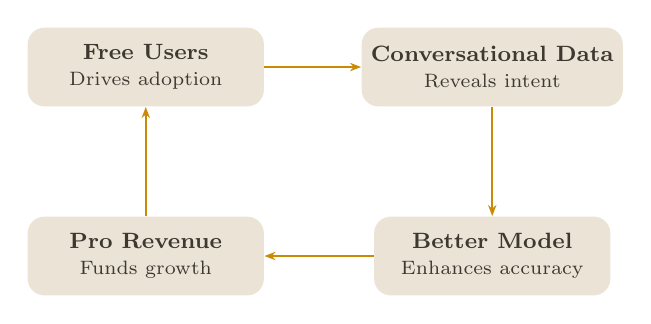
\begin{tikzpicture}[
  block/.style={rounded corners=6pt, fill=hcCard, text=hcText,
    minimum width=3cm, minimum height=1cm, align=center, font=\footnotesize},
  arr/.style={-{Stealth[length=4pt]}, thick, color=hcGold}
]
  \node[block] (consumers) at (-2.2,1.2) {\textbf{Free Users}\\{\scriptsize Drives adoption}};
  \node[block] (signal) at (2.2,1.2) {\textbf{Conversational Data}\\{\scriptsize Reveals intent}};
  \node[block] (model) at (2.2,-1.2) {\textbf{Better Model}\\{\scriptsize Enhances accuracy}};
  \node[block] (value) at (-2.2,-1.2) {\textbf{Pro Revenue}\\{\scriptsize Funds growth}};

  \draw[arr] (consumers) -- (signal);
  \draw[arr] (signal) -- (model);
  \draw[arr] (model) -- (value);
  \draw[arr] (value) -- (consumers);
\end{tikzpicture}
\end{center}

\vspace{4pt}
\textcolor{hcGoldLight}{\rule{\textwidth}{0.5pt}}
\vspace{4pt}

\textbf{Defensibility}\\[6pt]
\begin{description}\setlength{\itemsep}{2pt}
  \item[\goldtext{Data Asset}] \quad\phantom{...}Intention reveals buyer needs
  \item[\goldtext{Switching Costs}] \phantom{.}Transparency locks in trust
  \item[\goldtext{Network Effects}] \phantom{}Market prices against model
\end{description}
\end{frame}

% ─── SLIDE 6: Market Opportunity ─────────────────────────────
\begin{frame}{Market: The \$15B Forecast Layer}
\vspace{12pt}

\begin{center}
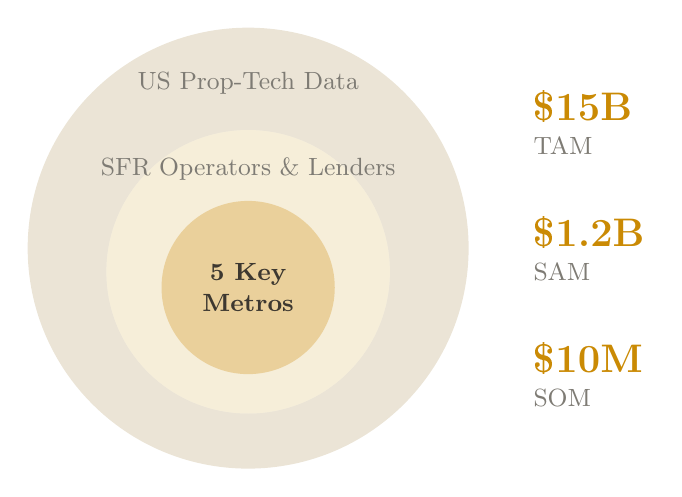
\begin{tikzpicture}
  % TAM
  \fill[hcCard] (0,0) circle (2.8cm);
  \node[text=hcMuted] at (0, 2.1) {\small US Prop-Tech Data};

  % SAM
  \fill[hcBg] (0,-0.3) circle (1.8cm);
  \fill[hcGoldLight!40] (0,-0.3) circle (1.8cm);
  \node[text=hcMuted] at (0, 1.0) {\small SFR Operators \& Lenders};

  % SOM
  \fill[hcGold!40] (0,-0.5) circle (1.1cm);
  \node[text=hcText, font=\small\bfseries, align=center] at (0, -0.5) {5 Key\\Metros};

  % Labels
  \node[text=hcGold, font=\Large\bfseries, anchor=west] at (3.5, 1.8) {\$15B};
  \node[text=hcMuted, font=\small, align=left, anchor=west] at (3.5, 1.3) {TAM};

  \node[text=hcGold, font=\Large\bfseries, anchor=west] at (3.5, 0.2) {\$1.2B};
  \node[text=hcMuted, font=\small, anchor=west] at (3.5, -0.3) {SAM};

  \node[text=hcGold, font=\Large\bfseries, anchor=west] at (3.5, -1.4) {\$10M};
  \node[text=hcMuted, font=\small, anchor=west] at (3.5, -1.9) {SOM};
\end{tikzpicture}
\end{center}

\vspace{4pt}
\begin{center}
\mutedtext{\scriptsize *TAM based on 8M+ investors. SOM reflects Year 3 target in initial metros.}
\end{center}
\end{frame}

% ─── SLIDE 7: Competitive Landscape ─────────────────────────
\begin{frame}{Landscape}
\vspace{6pt}

{\footnotesize
\begin{center}
\begin{tabular}{l c c c c}
\toprule
& \textbf{CoreLogic\textsuperscript{1}} & \textbf{HouseCanary\textsuperscript{2}} & \textbf{PropStream\textsuperscript{3}} & \goldtext{\textbf{Homecastr}} \\
\midrule
\textbf{Model} & Legacy ML & ML & Database & \goldtext{\textbf{Diffusion}} \\
\textbf{Output} & History & Value & Lists & \goldtext{\textbf{Forecast}} \\
\textbf{Forecasts?} & No & Point & No & \goldtext{\textbf{Bands}} \\
\textbf{Context} & None & Manual & Manual & \goldtext{\textbf{Automated}} \\
\textbf{Access} & Enterprise & Enterprise & Self-serve & \goldtext{\textbf{Self-serve}} \\
\textbf{Price} & Contract & Contract & \$99/mo & \goldtext{\textbf{Freemium}} \\
\bottomrule
\end{tabular}
\end{center}
}

\vspace{2pt}
{\scriptsize
\mutedtext{\textsuperscript{1}CoreLogic. \textsuperscript{2}HouseCanary. \textsuperscript{3}PropStream.}
}

\vspace{6pt}
\begin{center}
\goldtext{\textbf{Only foundation model forecasts}}\\
\goldtext{with explainable outputs and self-serve GTM.}
\end{center}
\end{frame}

% ─── SLIDE 8: Business Model ────────────────────────────────
\begin{frame}{Business Model}
\vspace{4pt}

\begin{columns}[T]
\begin{column}{0.58\textwidth}
\textbf{\large\goldtext{Target Customer}}\\[4pt]
\textbf{Individual real estate investors}\\in 5 high-growth metros\\[4pt]
\begin{itemize}\setlength{\itemsep}{2pt}
  \item Time exits with forward-looking data
  \item Underserved by enterprise tools
  \item Pay for edge over Zillow estimates
\end{itemize}
\end{column}
\begin{column}{0.40\textwidth}
\textbf{\large\goldtext{Target Unit Economics}}\\[6pt]
\begin{tabular}{l r}
\textbf{Pricing} & \$99/mo Operator \\
\textbf{Target LTV} & \textbf{\$1,188}\textsuperscript{*} \\
\textbf{Target CAC} & \textbf{\$150} \\
\textbf{LTV:CAC} & \textbf{8x} \\
\textbf{Payback} & \textbf{1.5 months} \\
\end{tabular}
\end{column}
\end{columns}

\vspace{6pt}
{\footnotesize
\begin{center}
\begin{tabular}{l l l l l}
\toprule
\textbf{Plan} & \textbf{Price} & \textbf{Target} & \textbf{Revenue} & \textbf{Value} \\
\midrule
Free & \$0 & 50K+ users & Lead Gen & Basic \\
\textbf{Operator} & \textbf{\$99/mo} & 1,700 subs & \textbf{\$2.0M} & \textbf{Bulk/API}\\
\bottomrule
\end{tabular}
\end{center}
}
\begin{center}
\mutedtext{\scriptsize *Assumes 12-month retention.}
\end{center}
\end{frame}

% ─── SLIDE 9: Go-to-Market ──────────────────────────────────
\begin{frame}{Go-to-Market}
\vspace{12pt}

\begin{center}
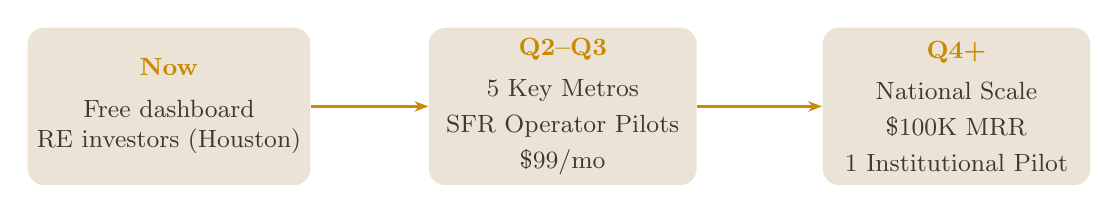
\begin{tikzpicture}[
  phase/.style={rounded corners=6pt, fill=hcCard, text=hcText,
    minimum width=3.4cm, minimum height=2cm, align=center, font=\small},
  arr/.style={-{Stealth[length=5pt]}, thick, color=hcGold}
]
  \node[phase] (p1) at (0,0) {
    \goldtext{\textbf{Now}}\\[4pt]
    Free dashboard\\RE investors (Houston)
  };
  \node[phase] (p2) at (5,0) {
    \goldtext{\textbf{Q2--Q3}}\\[4pt]
    5 Key Metros\\[2pt]
    SFR Operator Pilots\\[2pt]
     \$99/mo
  };
  \node[phase] (p3) at (10,0) {
    \goldtext{\textbf{Q4+}}\\[4pt]
    National Scale\\[2pt]
    \$100K MRR\\[2pt]
    1 Institutional Pilot
  };

  \draw[arr] (p1) -- (p2);
  \draw[arr] (p2) -- (p3);
\end{tikzpicture}
\end{center}

\vspace{12pt}
\begin{center}
\mutedtext{\begin{itemize}\setlength{\itemsep}{10pt}
  \item \textbf{Programmatic SEO}\\\mutedtext{Capture high-intent search traffic}
  \item \textbf{Broker-Client Share Loops}\\\mutedtext{Agents send forecasts to leads}
  \item \textbf{Index against Forecasts}\\\mutedtext{SEO for "Will [Address] appreciate?"}
\end{itemize}}
\end{center}
\end{frame}

% ─── SLIDE 9: Traction ──────────────────────────────────────
\begin{frame}{Where We Are}
\vspace{20pt}

\begin{center}
\statbox{14\%}{Median Error}
\hfill
\statbox{4yr}{Forecast Horizon}
\hfill
\statbox{Live}{Dashboard}
\hfill
\statbox{Ready}{API}
\end{center}

\vspace{20pt}

\begin{itemize}
  \item Houston metro: 1M+ properties indexed
  \item Diffusion-based foundation model producing forecast bands
  \item AI voice agent for hands-free exploration
\end{itemize}
\end{frame}

% ─── SLIDE 1: Title ────────────────────────────────────────────
\begin{frame}[plain]{Team}
\vspace{4pt}

\begin{columns}[c]
\begin{column}{0.25\textwidth}
\centering
\begin{tikzpicture}
  \node[circle, inner sep=0pt, minimum size=2.5cm, path picture={
    \node at (path picture bounding box.center) {\includegraphics[width=2.5cm]{dhl.jpg}};
  }] {};
\end{tikzpicture}
\end{column}
\begin{column}{0.70\textwidth}
{\Large\bfseries\color{hcGold} Daniel Hardesty Lewis}\\[4pt]
{\large Founder \& CEO}\\[2pt]
\mutedtext{\small \href{https://linkedin.com/in/dhardestylewis}{linkedin.com/in/dhardestylewis}}
\end{column}
\end{columns}

\vspace{8pt}

\begin{columns}[T]
\begin{column}{\textwidth}
\begin{itemize}\setlength{\itemsep}{3pt}
  \item \textbf{Founder, Summit Geospatial}\\\mutedtext{Highest quality terrain in Texas}
  \item \textbf{Sr. Data Scientist, TACC}\\\mutedtext{Principal on \$40M resiliency project}
  \item \textbf{Scientific ML}\\\mutedtext{Bagnold Medal Research Contributor}
  \item \textbf{Teaching}\\\mutedtext{ML for Petrobras Geoscientists}
\end{itemize}
\end{column}
\end{columns}
\end{frame}

% ─── SLIDE 11: The Ask ──────────────────────────────────────
\begin{frame}[c]
\vspace{4pt}

\begin{center}
{\fontsize{36}{42}\selectfont\bfseries\color{hcGold} Raising \$1M}\\[8pt]
{\large Pre-Seed}
\end{center}

\vspace{10pt}

\begin{columns}[T]
\begin{column}{0.49\textwidth}
\textbf{Use of Funds}\\[6pt]
\begin{itemize}\setlength{\itemsep}{6pt}
  \item \textbf{ML Engineer}\\\mutedtext{transfer learning to new markets}
  \item \textbf{GTM / Sales}\\\mutedtext{scale to 1,700+ Operators}
  \item \textbf{Data, compute}\\\mutedtext{CoreLogic, GPUs, 5 metros}
\end{itemize}
\end{column}
\begin{column}{0.48\textwidth}
\textbf{18-Month Milestones}\\[6pt]
\begin{itemize}\setlength{\itemsep}{4pt}
  \item 5 metros, 8M+ properties
  \item \$50K MRR
  \item 1 institutional pilot or LOI
\end{itemize}
\end{column}
\end{columns}

\vspace{4pt}
\begin{center}
\href{https://homecastr.com}{\goldtext{homecastr.com}} \quad|\quad \href{mailto:daniel@homecastr.com}{\mutedtext{daniel@homecastr.com}}
\end{center}
\vfill
\begin{center}
% ─── SLIDE 12: Contact / Title Repeat ────────────────────────
\usebackgroundtemplate{\includegraphics[width=\paperwidth,height=\paperheight]{title_bg.png}}
\begin{frame}[plain]
\vfill
\begin{center}
{\buildingicon}\quad{\fontsize{42}{48}\selectfont\bfseries\color{hcGold} Homecastr}\\[16pt]
{\Large\color{hcText} The foundation model for residential real estate}\\[24pt]
\mutedtext{Pre-Seed Deck \quad|\quad 2026}\\[8pt]
\mutedtext{\small Live Demo: \href{https://homecastr.com}{\textcolor{hcGold}{\textbf{homecastr.com}}}}
\end{center}
\vfill
\end{frame}

\end{document}
